%
% !TeX root =./main.tex
% !TeX spellcheck = en_US


For our study we consider the road network of the state of Carinthia, Austria.
We base our study on data that is available from OSM \cite{OpenStreetMap}.
% For now, we consider the \textit{higher level road network} in Carinthia, Austria,
% i.e., \textit{A}, \textit{S}, \textit{L}, \textit{B}, in the  form of a matrix.

We use the \emph{R} programming language \cite{RVienna} to extract that data from
\emph{Overpass} API we use the \texttt{osmdata} R package \cite{osmdataR20221}.


\begin{figure}[!ht]
  \centering
  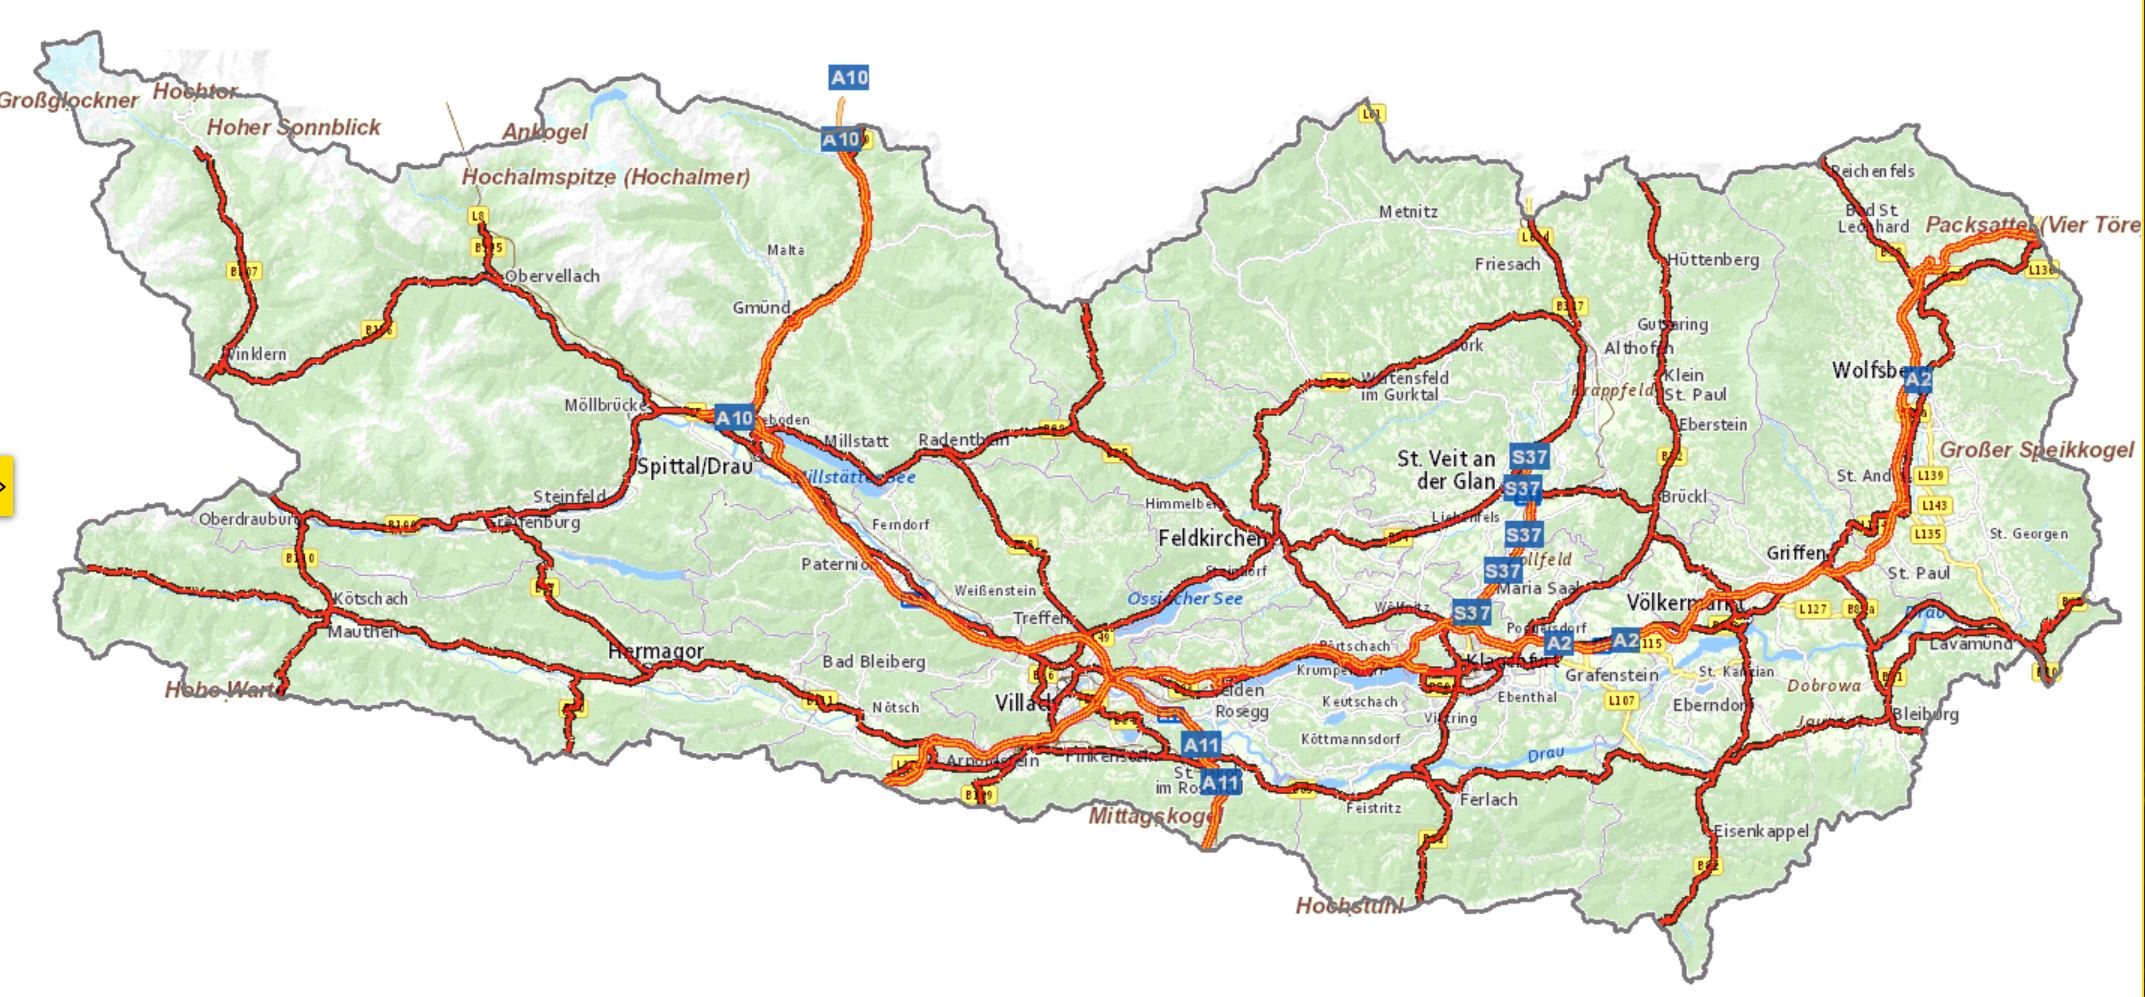
\includegraphics[width=0.9\textwidth]{map.jpg}
  \caption{Overview of the higher level road network in Carinthia.}
  \label{fig:higher level}
\end{figure}


\subsection{Road Network and Levels}
To get the road network we query the OSM \texttt{key}$=$\textit{highway}. We consider the
assigned values indicate the importance of the highway within the road network.
This classification is typically highly correlated to the official (legal) classification
but is not obligated to adhere to them. In our analysis we consider the
\texttt{values}$=$
\textit{'motorway', 'trunk', 'primary', 'secondary', 'tertiary', 'motorway\_link', 'trunk\_link', 'primary\_link', 'secondary\_link', 'tertiary\_link'}

\subsection{Maximum Road Gradients}

\begin{figure}[!ht]
  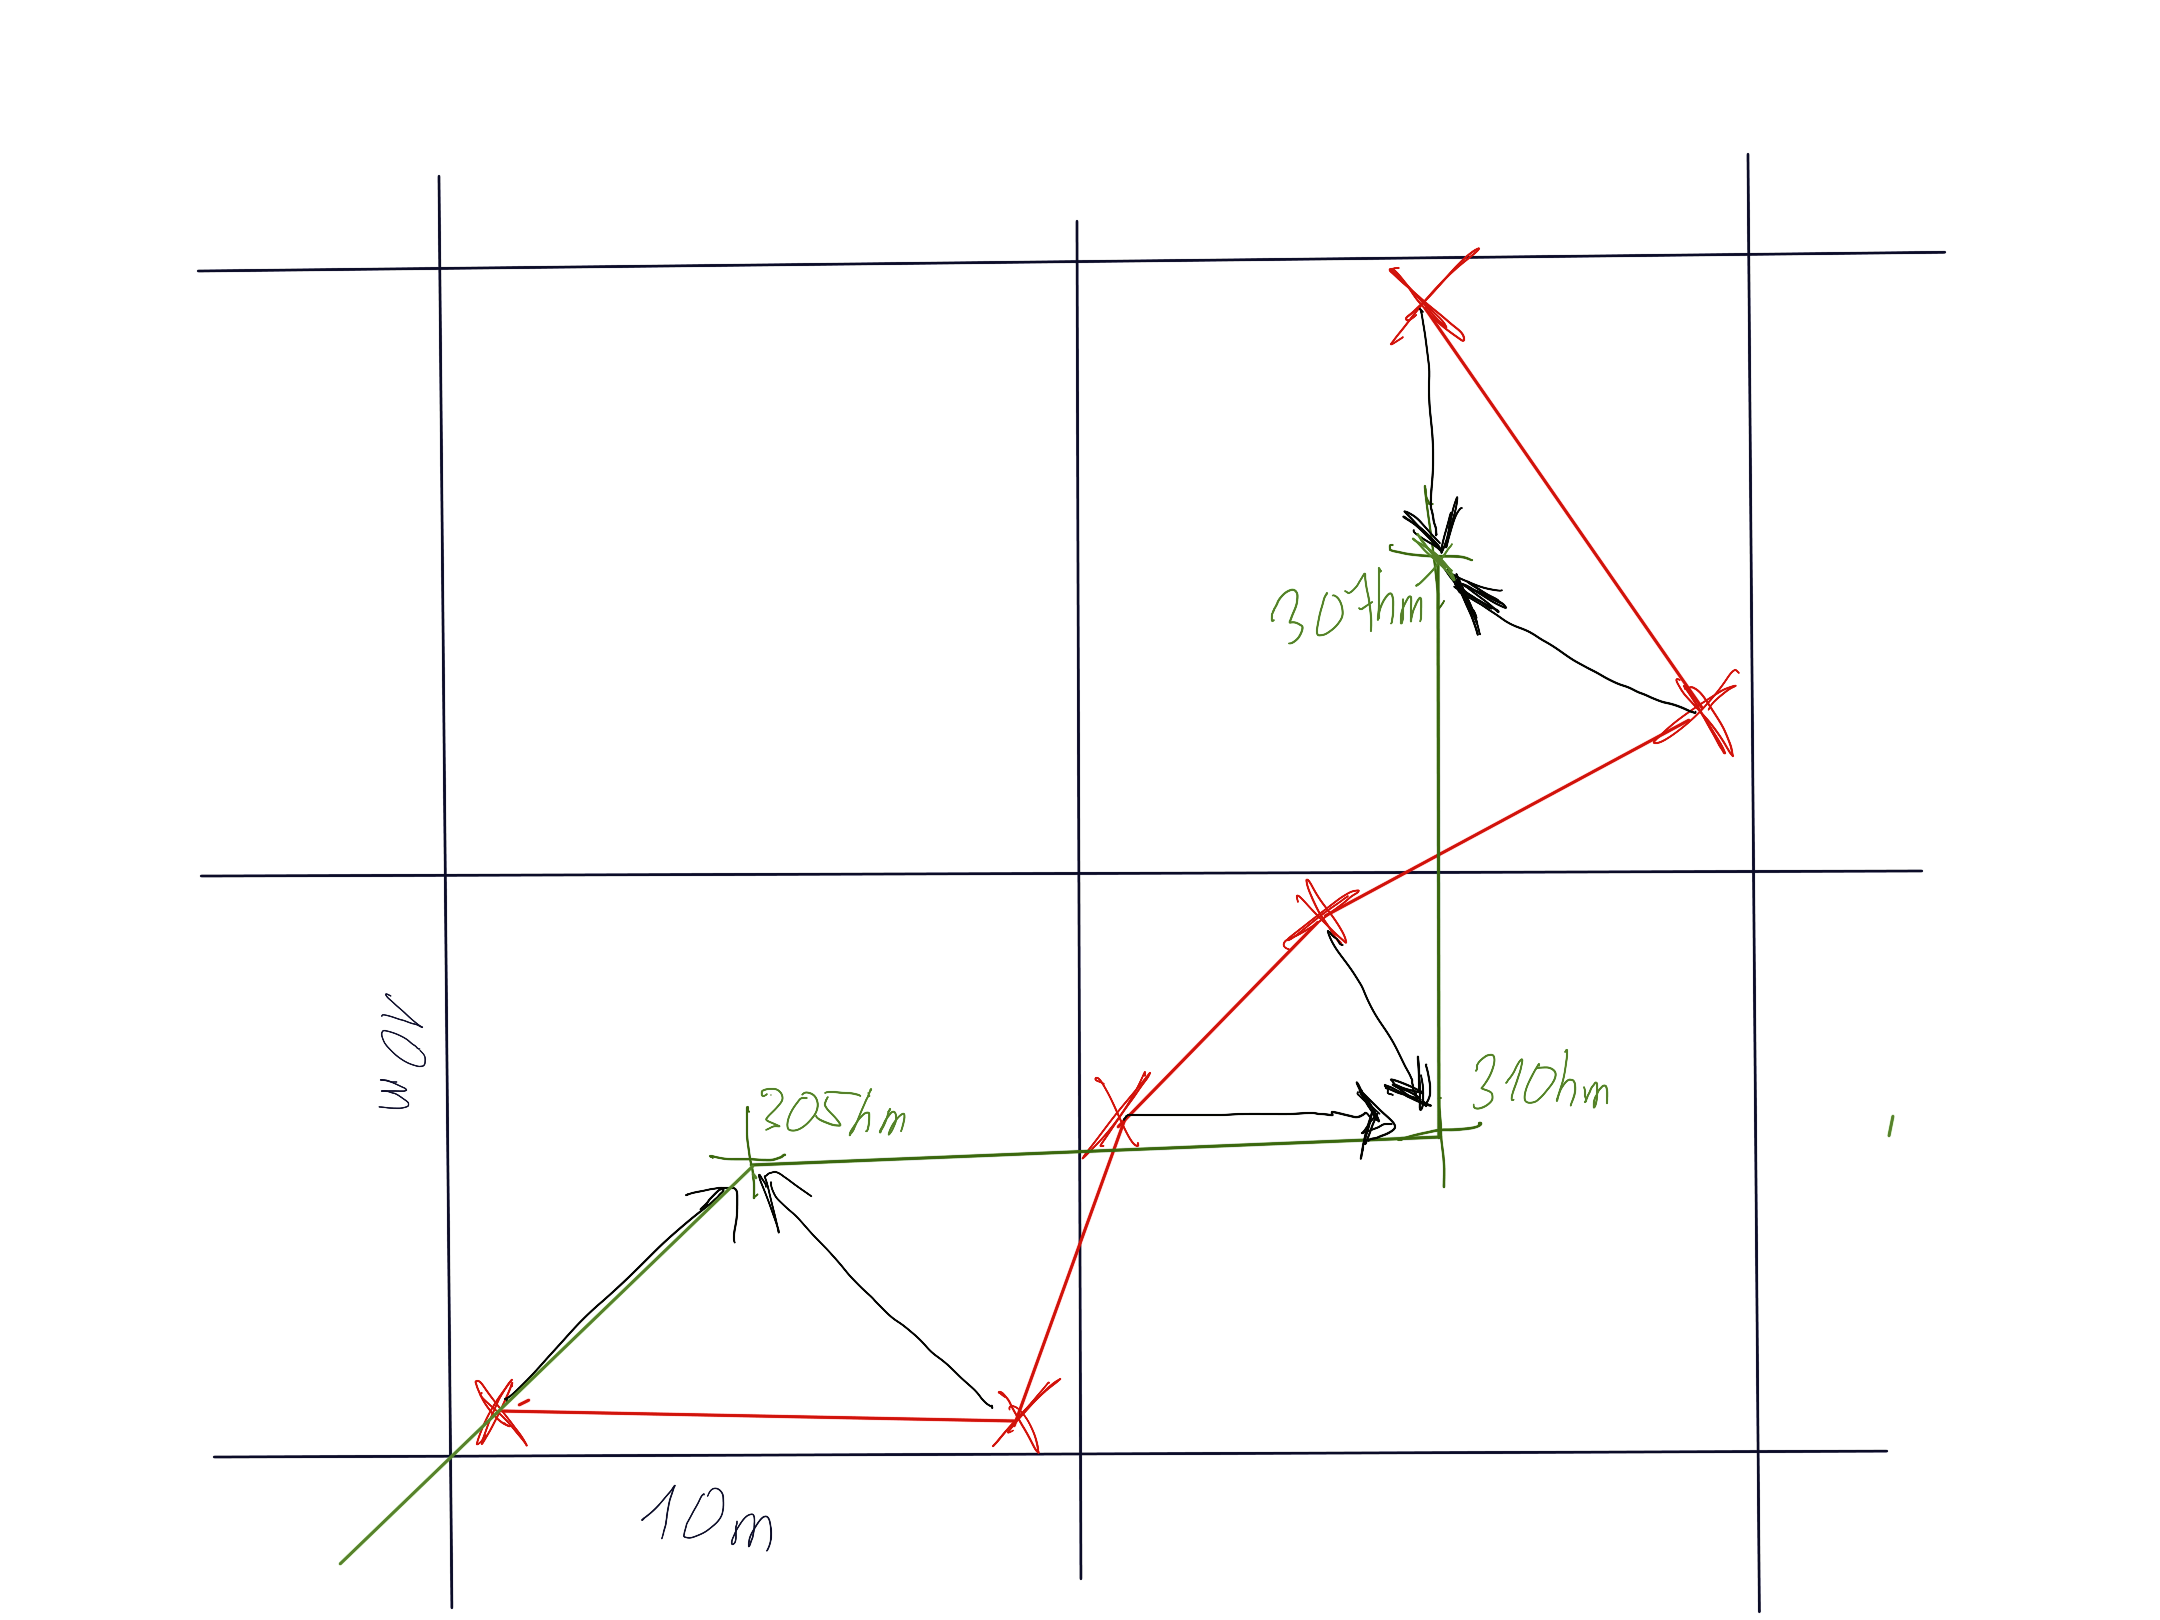
\includegraphics[width=0.9\textwidth]{./figures/mapping.png}
  \caption{Illustration of how a linestring is mapped to the grid that gives the elevation data.}
  \label{fig:mapelev}
\end{figure}
% https://civilnoteppt.com/6-types-of-classification-of-gradient-ruling-limiting-exceptional-minimum-average-and-floating-gradient/
% https://www.civillead.com/road-gradient/


\subsection{Bridge Weight Capacities}
Bridges are extracted by querying the \texttt{key}$=$\textit{bridge}. The tag \textit{maxweight}
tells as the maximal carrying capacity of the bridge. In case that no the field is empty,
following the rule of thump, there is now restriction for road legal vehicles, and
a weight restriction of $60t$ (or more is assumed).
We map the bridges to the road segment using the \texttt{???} package.


\subsection{Sample Transport Request}

\begin{table}[!ht]
  \caption{Overview of the transport request considered in the analysis.}
  \label{tab:request}
  \centering
\begin{tabular}{l|llll|l}
Type  & $w(r)$  & $g(r)$  & $o$  & $d$ & Description\\ \hline\hline
Super heavy  & 58t  & 0.08 & Thörl-Maglern  & Villach (Industriegebiet) &  MAN TGX D3876 (387kw)\\
&&&&& + Goldhofer TN-L Flatbed Trailer
\\ \hline
\end{tabular}
\end{table}


\begin{table}[!ht]
  \caption{Sample transport requests.}
  \label{tab:sample}
  \centering
\begin{tabular}{ll|ll|ll|l}
  \hline
 \multicolumn{2}{c}{tractor} &  \multicolumn{2}{c}{trailer}  &   \multicolumn{2}{c}{load}  &total\\
 type & weight & type & weight &  description & weight \\ \hline
 Mercedes-Benz  & 10.32t  & Goldhofer  & 16.85t & construction machine & 48.3t   & 75.5t\\
 MAN  & 14.50  & Goldhofer  & 60.0t & part of hydr. press & 112.5t   & 187t\\
 MAN  & 14.01  & Scheurle  & 60.0t & not known & 65.72t   & 145t\\

  \hline
\end{tabular}
\end{table}



\begin{figure}[!ht]
  \centering
  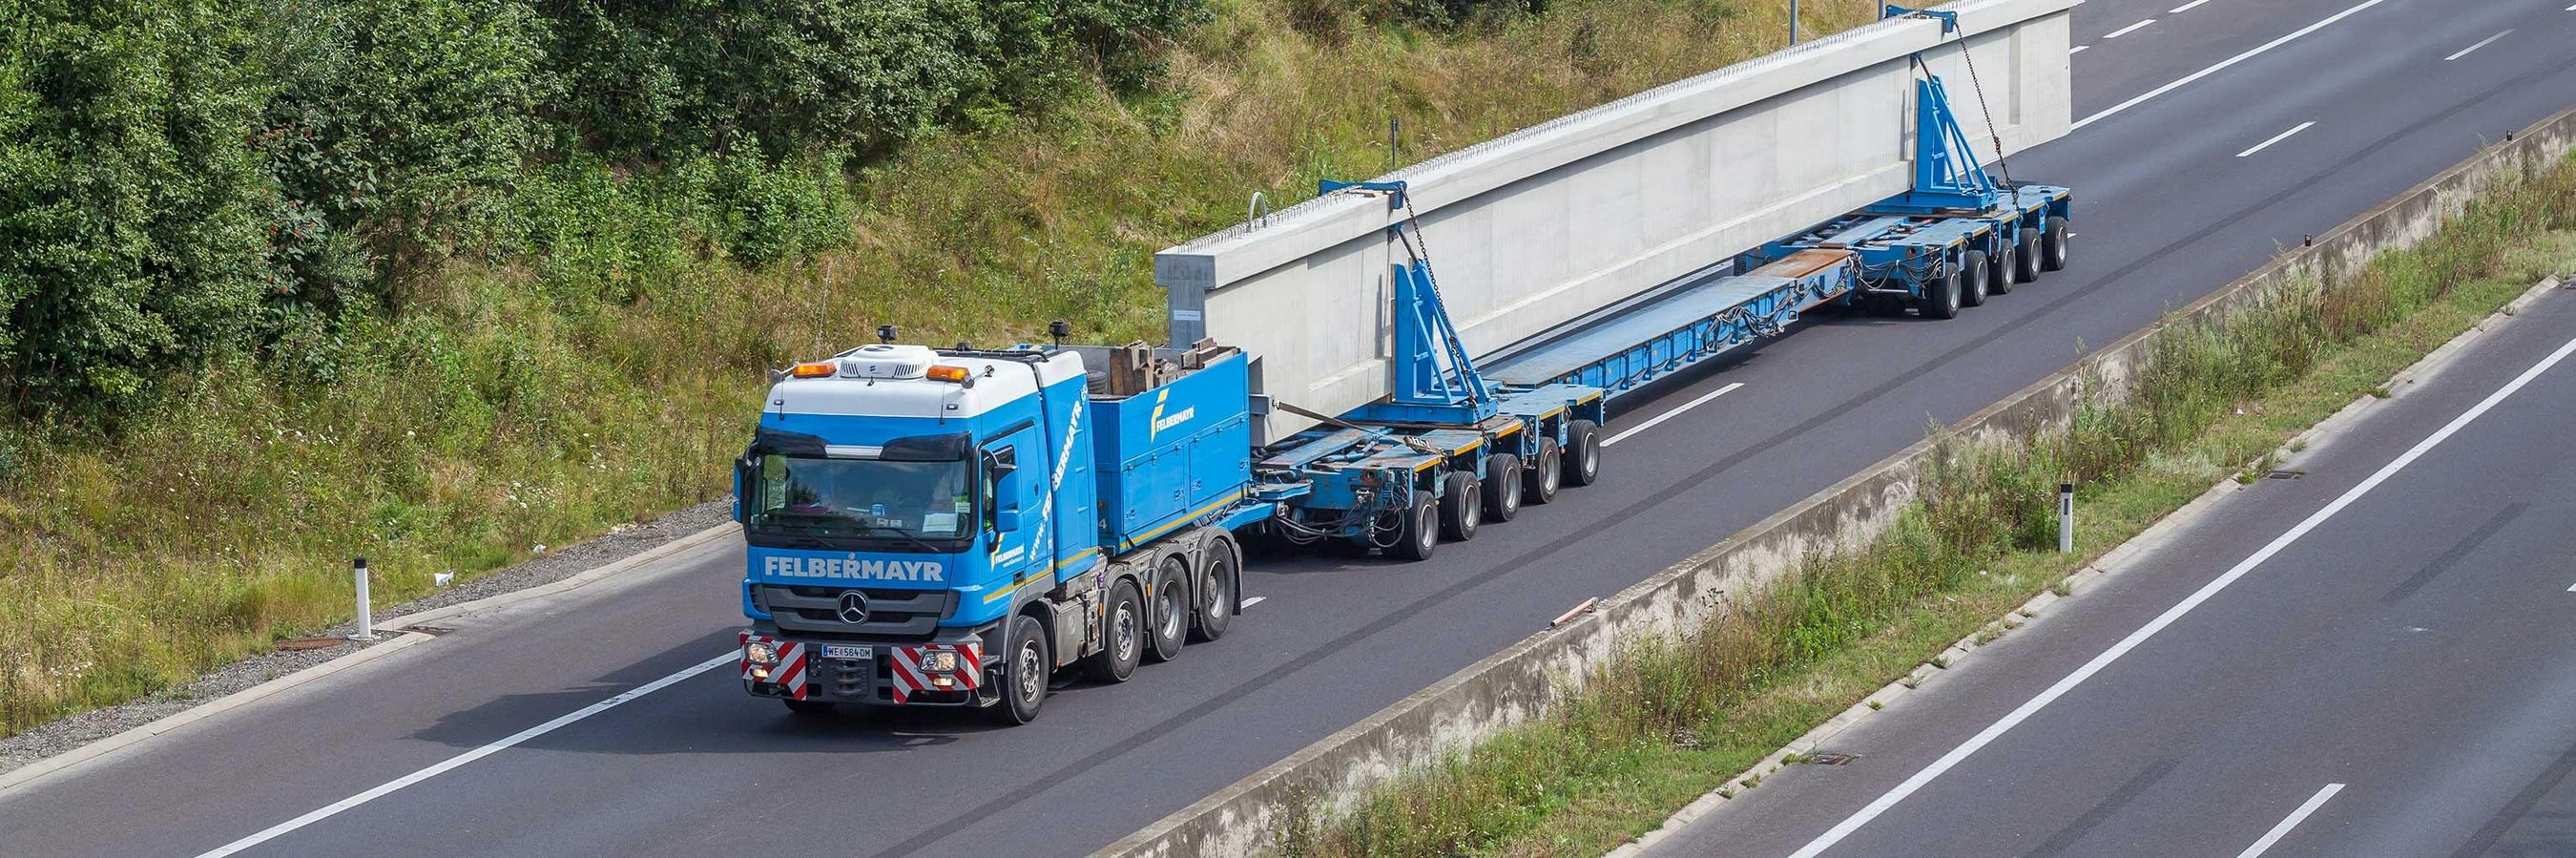
\includegraphics[width=0.5\textwidth]{./figures/felbert.jpg}
  \caption{\ohc transport on a motorway.}
  \label{fig:truck}
\end{figure}
